\documentclass{article}
\usepackage{graphicx}

\begin{document}

\title{Supplementary material for ``Visualization methods for RNA-sequencing data analysis"}
\author{Lindsay Rutter}

\maketitle

\begin{figure}[!p]
\centerline{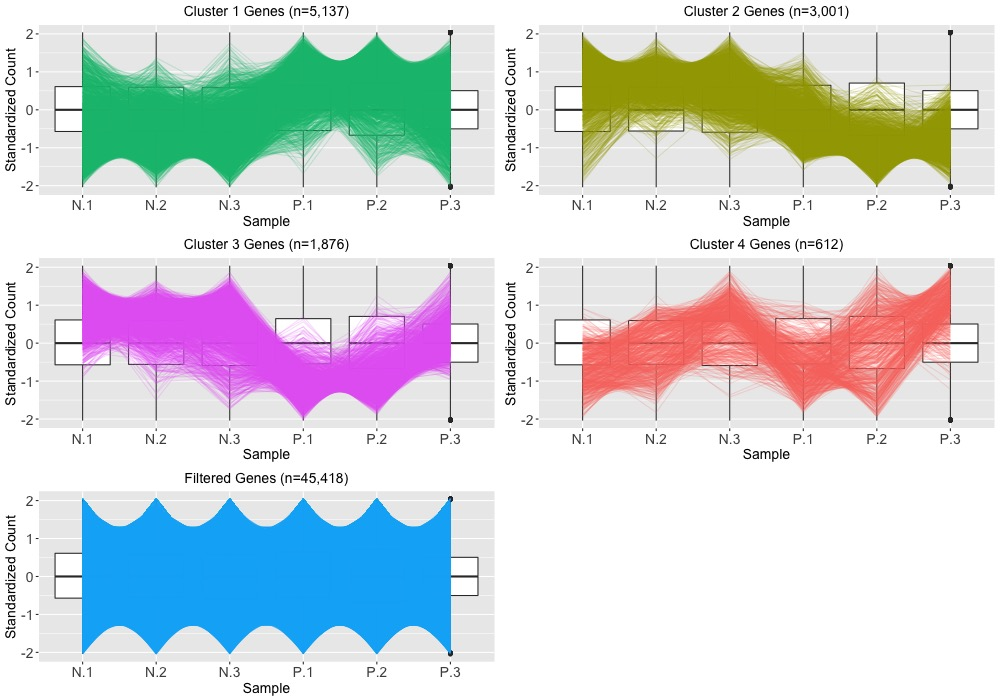
\includegraphics[width=\columnwidth]{/Users/lindz/JDSPaper/Bioinformatics/Pictures/FilterNotSig/ClusteringdataFDR05/NP4.jpg}}
\caption{Example application of parallel coordinate plots using the iron-metabolism soybean dataset. We filtered genes with low means and/or variance, performed a hierarchical clustering analysis with a cluster size of four, and visualized the results using parallel coordinate lines. Most non-filtered genes were in Clusters 1 and 2, which both showed overexpression in one treatment and underexpression in the other treatment. The genes in Cluster 4 mostly showed messy patterns with low signal to noise ratios. Interestingly, Cluster looked similar to Cluster 2 (large values for group N and small values for group P), except for unexpectedly large values for the third replicate of group P.
\label{suppNonSigCluster}}
\end{figure}

\begin{figure}[!p]
\centerline{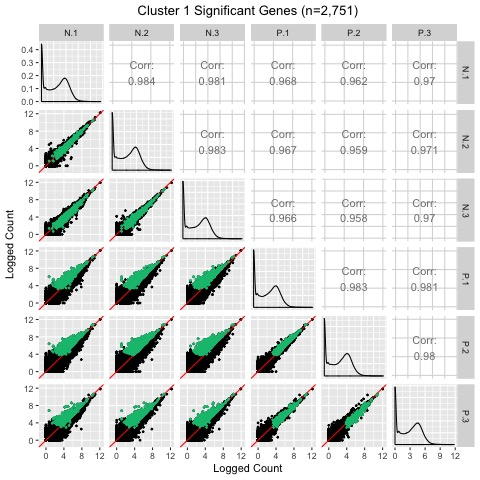
\includegraphics[width=\columnwidth]{/Users/lindz/JDSPaper/Bioinformatics/Pictures/FilterNotSig/Clustering_data_FDR_05/N_P_Sig_SM_4_1.jpg}}
\caption{Example of assessing DEG calls from a model with a scatterplot matrix using the iron-metabolism soybean dataset. There were 2751 significant genes in Cluster 1 after performing a hierarchical clustering analysis with a cluster size of four. These significant genes are overlaid in green over the scatterplot matrix. They follow the expected patterns of differential expression with most green points falling along the \textit{x=y} line in the scatterplots between replicates, but deviating from the \textit{x=y} line in the scatterplots between treatments. The deviation consistently demonstrates higher expression in the P group than the N group. Hence, these green points seem to represent genes that were expressed higher in the P group in a statistically-significant manner, which lines up with what we saw in the parallel coordinate plots in Figure 2 of the paper.
\label{suppSMCluster1}}
\end{figure}

\begin{figure}[!p]
\centerline{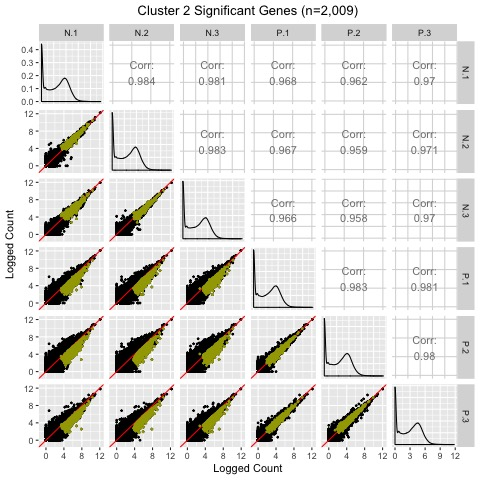
\includegraphics[width=\columnwidth]{/Users/lindz/JDSPaper/Bioinformatics/Pictures/FilterNotSig/Clustering_data_FDR_05/N_P_Sig_SM_4_2.jpg}}
\caption{Caption
\label{suppSMCluster2}}
\end{figure}
  
\begin{figure}[!p]
\centerline{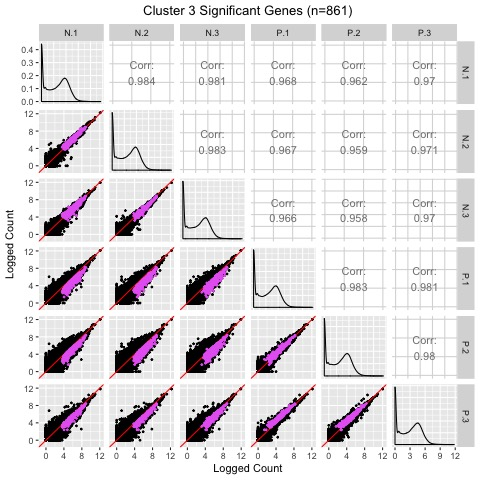
\includegraphics[width=\columnwidth]{/Users/lindz/JDSPaper/Bioinformatics/Pictures/FilterNotSig/Clustering_data_FDR_05/N_P_Sig_SM_4_3.jpg}}
\caption{Caption
\label{suppSMCluster3}}
\end{figure}  
  
\begin{figure}[!p]
\centerline{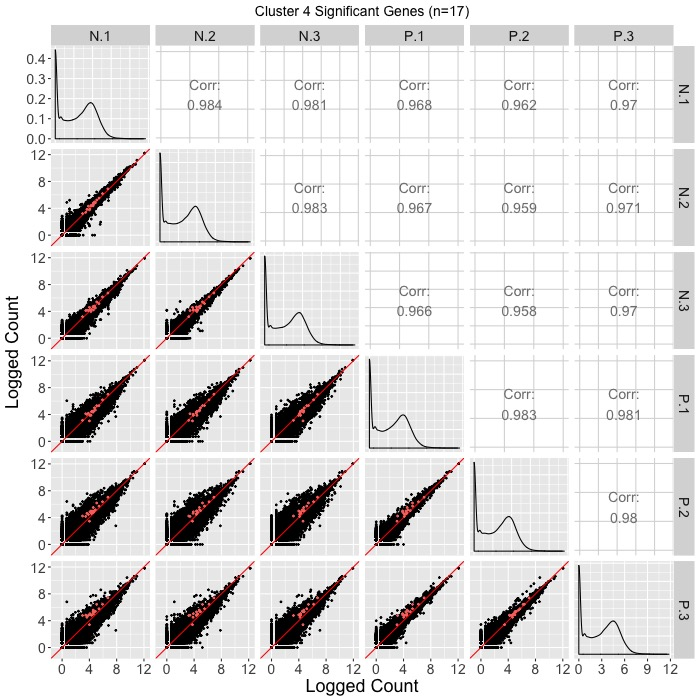
\includegraphics[width=\columnwidth]{/Users/lindz/JDSPaper/Bioinformatics/Pictures/FilterNotSig/Clustering_data_FDR_05/N_P_Sig_SM_4_4.jpg}}
\caption{Caption
\label{suppSMCluster4}}
\end{figure}  
  
\begin{figure}[!p]
\centerline{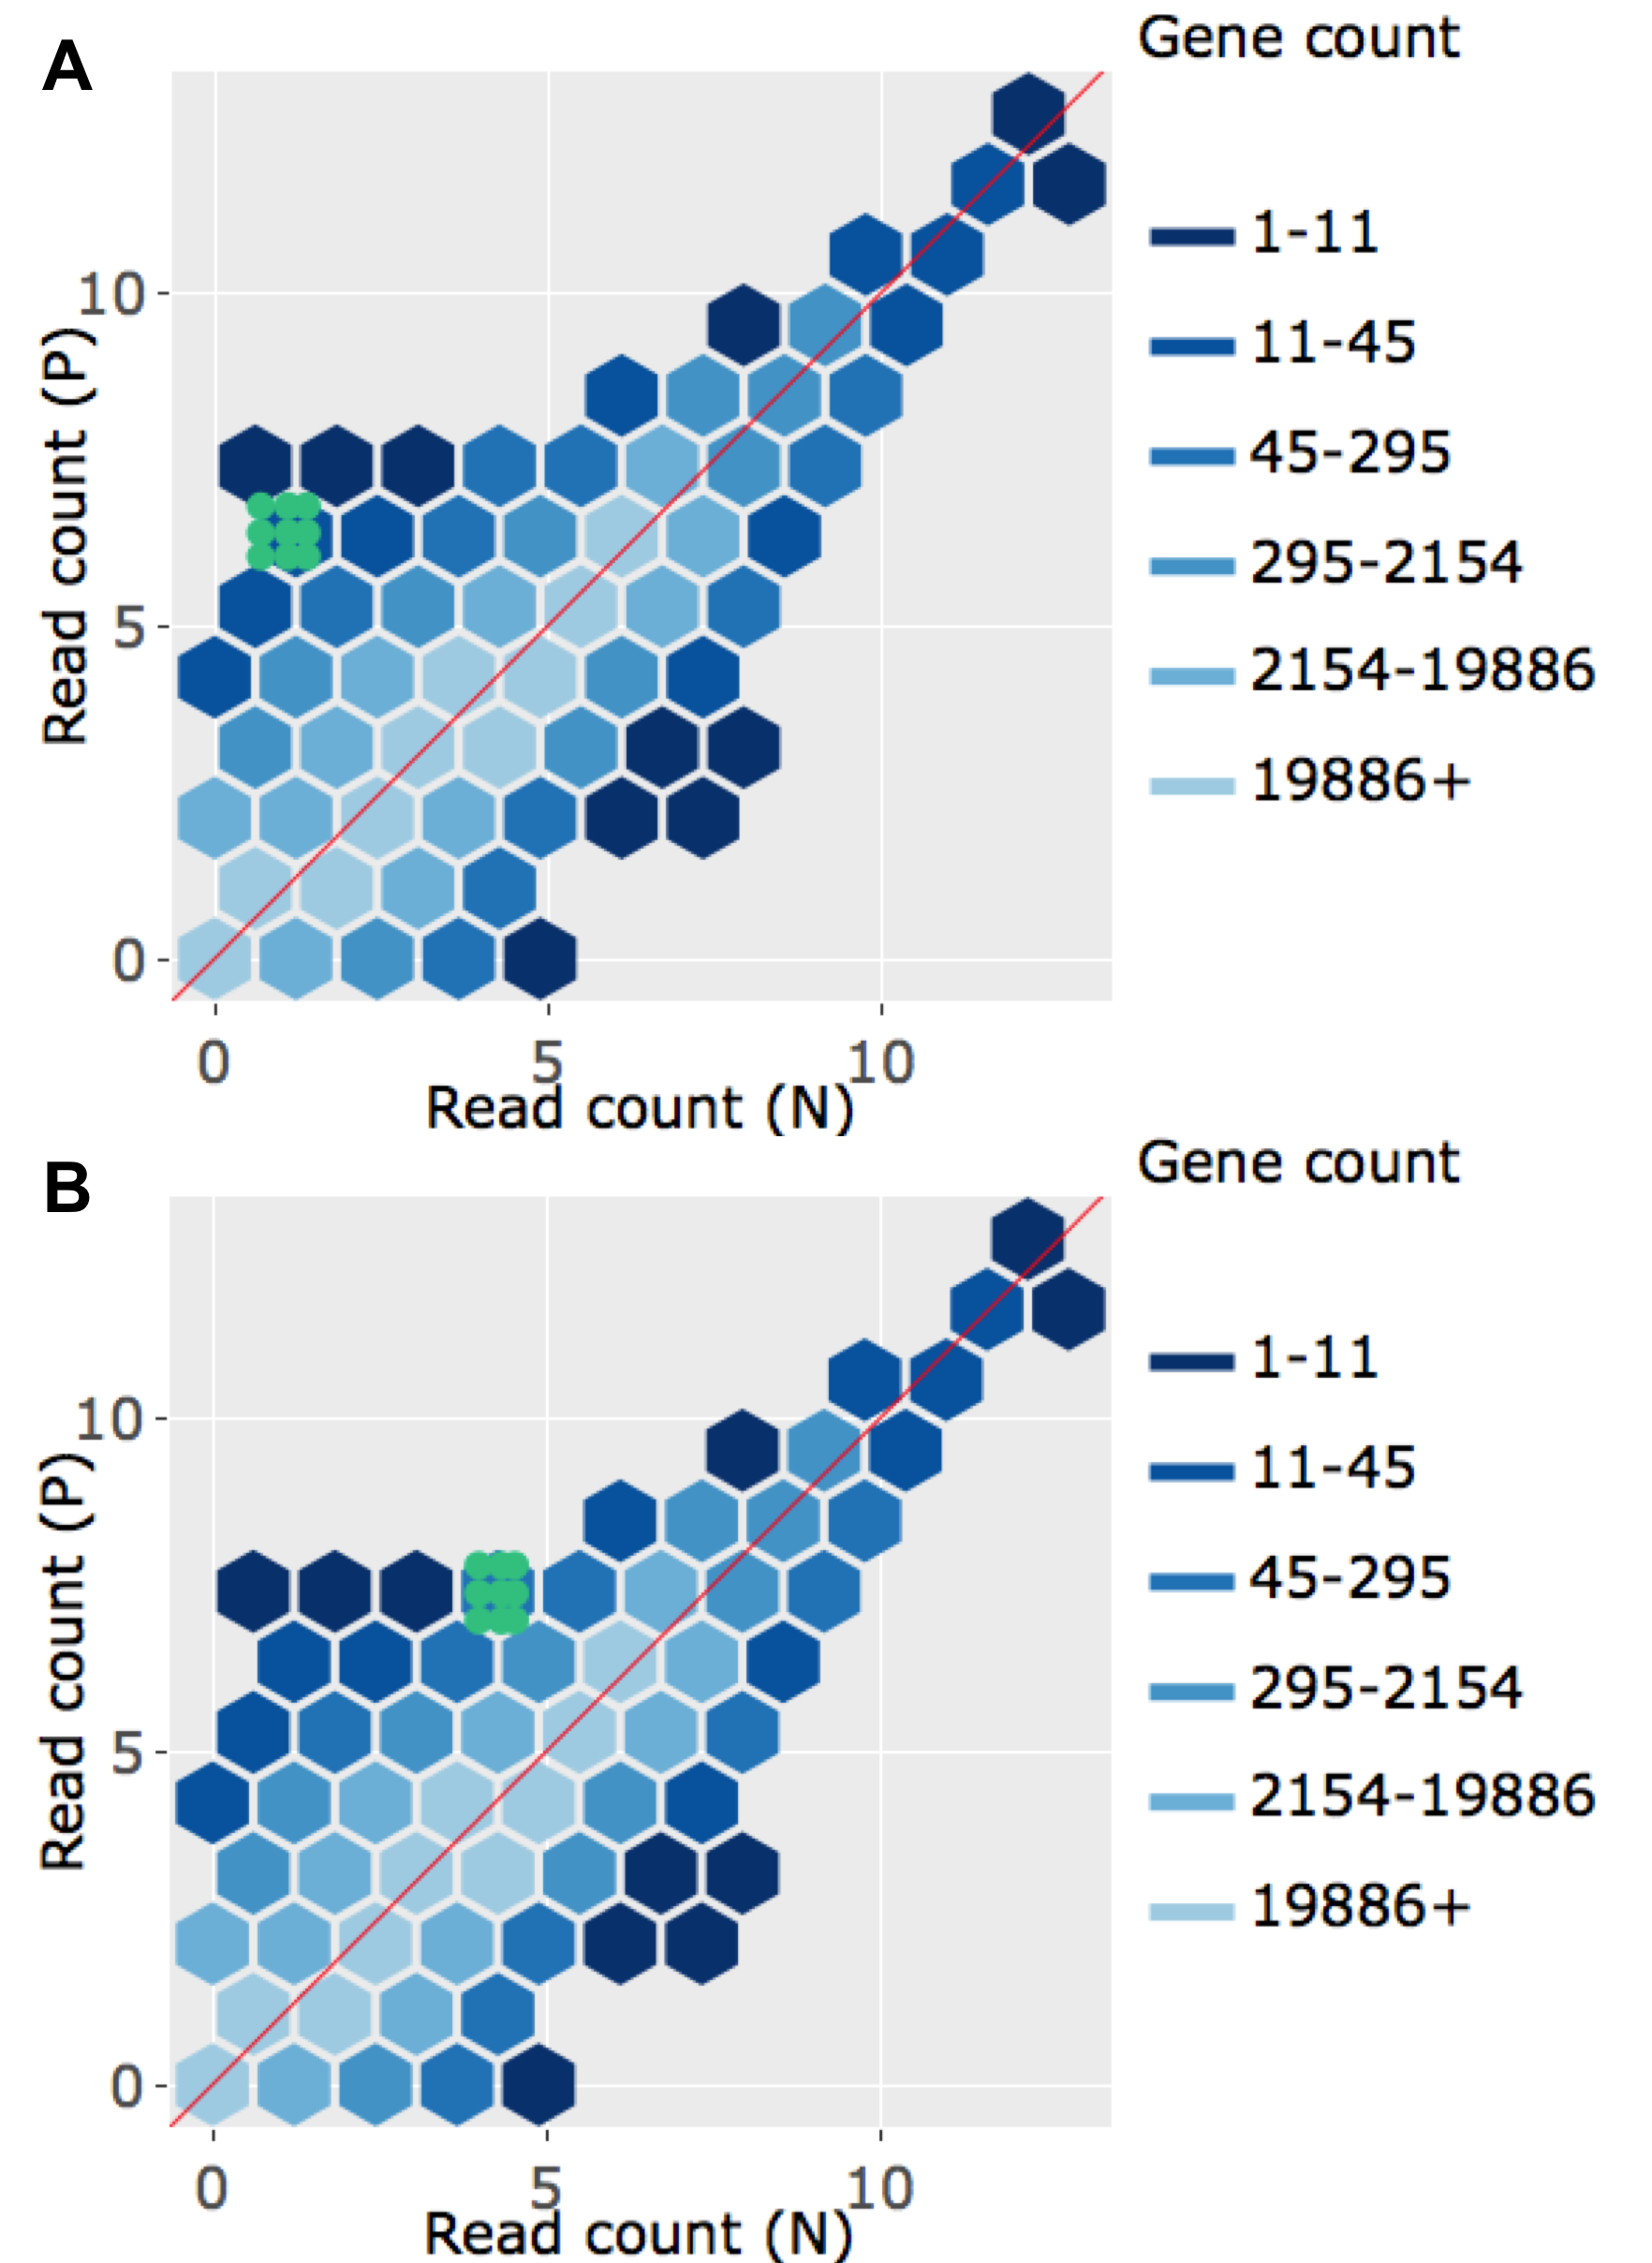
\includegraphics[width=0.7\columnwidth]{/Users/lindz/JDSPaper/Bioinformatics/Pictures/litrePlots/N_P/litreCluster1.png}}
\caption{Caption
\label{litreCluster1}}
\end{figure}   

\end{document}